\chapter{运行实例}

\begin{figure}[htbp]
\centerline{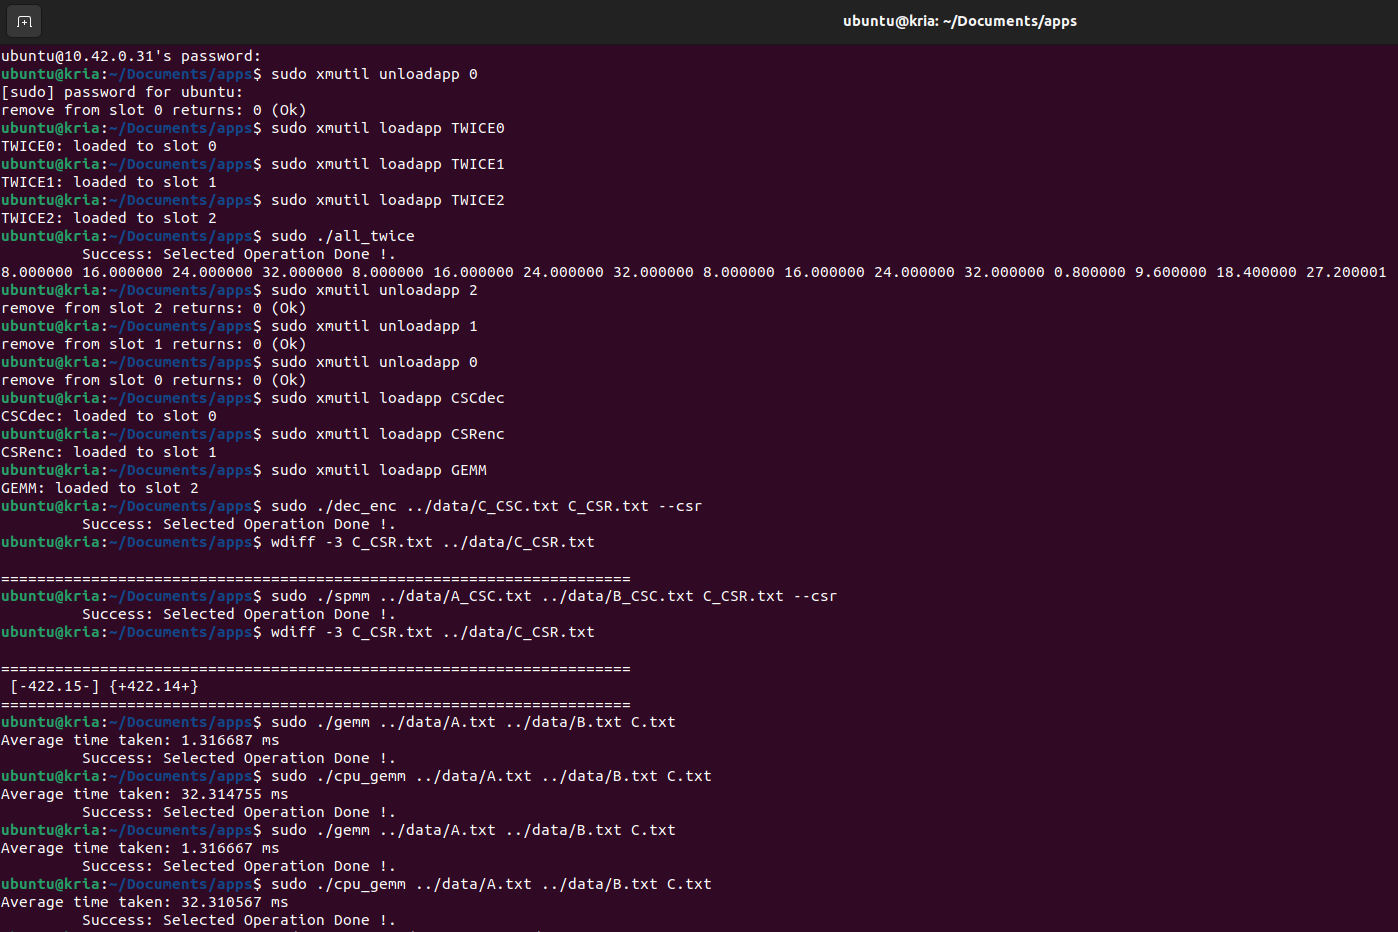
\includegraphics[width=\columnwidth]{figures/run.png}}
\caption{128\texttimes{}128矩阵乘法的运行实例。}
\label{fig:run}
\end{figure}

在图~\ref{fig:run} 中,我们先用 \verb|xmutil| 命令装载了三个 \verb|TWICE| RM,它们的功能是将输入流翻倍后输出。
我们随后执行 \verb|all_twice| 应用以测试RM间的互联,此应用定义RP\_0的输入为DDR,RP\_0输出为RP\_1的输入,
RP\_1输出为RP\_2的输入,RP\_2的输出为DDR,也就是将最开始的输入翻8倍后输出。

我们接下来卸载三个 \verb|TWICE| RM,装载 \verb|CSCdec|(CSC矩阵解压RM),\verb|CSRenc|(CSR矩阵压缩RM),\verb|GEMM|(稠密矩阵乘法RM)。
\verb|dec_enc| 应用将 \verb|CSCdec| 的输出连接 \verb|CSRenc| 的输入,实现CSC格式转化为CSR格式。\verb|spmm| 应用执行稀疏矩阵乘法,其输入为2个CSC矩阵,输出为CSR矩阵。
\verb|wdiff| 工具用于比对FPGA输出与真实值。\verb|gemm| 和 \verb|cpu_gemm| 应用分别测试FPGA和CPU上稠密矩阵乘法的运行耗时。

\chapter{稠密矩阵乘法加速}

\begin{table}[htbp]
\caption{不同矩阵大小下的加速比(12\texttimes{}12脉动阵列分块)}
\centering
\begin{tabular}{|c|c|c|c|}
\hline
\textbf{矩阵大小} & \textbf{CPU耗时} & \textbf{FPGA耗时} & \textbf{加速比} \\ \hline
12\texttimes{}12 & 0.015 & 0.012 & 1.3\texttimes{} \\ \hline
36\texttimes{}36 & 0.37 & 0.052 & 7.1\texttimes{} \\ \hline
60\texttimes{}60 & 1.7 & 0.17 & 10\texttimes{} \\ \hline
96\texttimes{}96 & 7.3 & 0.56 & 13\texttimes{} \\ \hline
120\texttimes{}120 & 15 & 1.0 & 15\texttimes{} \\ \hline
128\texttimes{}128 & 32 & 1.3 & 25\texttimes{} \\ \hline
\end{tabular}
\label{tab:speedup}
\end{table}

表~\ref{tab:speedup} 展示了对各种矩阵大小获得的加速比。

\chapter{复现说明}

\begin{table}[htbp]
\caption{编译环境}
\centering
\begin{tabular}{lc}
\toprule
OS & Ubuntu 22.04.5 LTS \\
CPU & Intel Core i9-13900HX \\
Memory & 62.6 GiB \\
\bottomrule
\end{tabular}
\label{tab:env}
\end{table}

HLS代码由Vitis 2022.1综合成RTL IP,随后用Vivado 2022.1执行综合、实现和比特流生成,运行环境如表~\ref{tab:env} 所示。
在此环境下,Vivado流程需运行30分钟并占用55 GiB内存。若希望减小内存占用,可修改流程的并行线程数量。
同时,我们在 \url{github.com/fjtcin/dfx-3rp-bin} 提供了生成的二进制文件,可直接使用。

KV260的型号为 \verb|xck26-sfvc784-2LV-c|。
